\section{Preliminaries for the Implementation}
\label{sec:prelim}

%%\textbf{Background Information on Toolsuite}
\danielle{My suggestion is to place this at the front of the implementation section. It just seems like it is taking longer to get to the interesting part of the paper by having it here.}

The algorithms in this paper are implemented in the Safety Annex for the Architecture Analysis and Design Language (AADL) and require the Assume-Guarantee Reasoning Environment (AGREE)~\cite{NFM2012:CoGaMiWhLaLu} to annotate the AADL model in order to perform verification using the back-end model checker \jkind~\cite{2017arXiv171201222G}. 

\textbf{Architecture Analysis and Design Language}
We are using the Architectural Analysis and Design Language (AADL) to construct system architecture models of performance-critical, embedded, real-time systems~\cite{AADL_Standard,FeilerModelBasedEngineering2012}. %An AADL model describes a system in terms of a hierarchy of components and their interconnections, where each component can either represent a logical entity (e.g., application software functions, data) or a physical entity (e.g., buses, processors). 
Language annexes to AADL provide a richer set of modeling elements for various system design and analysis needs, and the language definition is sufficiently rigorous to support formal analysis tools that allow for early phase error/fault detection. 

\textbf{Compositional Analysis} 
One way to structure compositional verification is hierarchically: layers of the system architecture are analyzed independently and their composition demonstrates a system property of interest. Compositional verification partitions the formal analysis of a system architecture into verification tasks that correspond into the decomposition of the architecture~\cite{clarke1989compositional}.  A proof consists of demonstrating that the system property is provable given the contracts of its direct subcomponents and the system assumptions~\cite{cofer2012compositional,clarke1989compositional}. When compared to monolithic analysis (i.e., analysis of the flattened model composed of all components), the compositional approach allows the analysis to scale to much larger systems~\cite{NFM2012:CoGaMiWhLaLu,heckel1998compositional,cofer2012compositional}.

\textbf{Assume Guarantee Reasoning Environment}
The Assume Guarantee Reasoning Environment (AGREE) is a tool for formal analysis of behaviors in AADL models and supports compositional verification~\cite{NFM2012:CoGaMiWhLaLu}.  It is implemented as an AADL annex and is used to annotate AADL components with formal behavioral contracts. Each component's contracts includes assumptions and guarantees about the component's inputs and outputs respectively. AGREE translates an AADL model and the behavioral contracts into Lustre~\cite{Halbwachs91:IEEE} and then queries the \jkind model checker to conduct the back-end analysis~\cite{2017arXiv171201222G}. 

\textbf{JKind}
JKind is an open-source industrial infinite-state inductive model checker for safety properties~\cite{2017arXiv171201222G}. Models and properties in JKind are specified in Lustre~\cite{Halbwachs91:IEEE}, a synchronous dataflow language, using the theories of linear real and integer arithmetic. JKind uses SMT-solvers to prove and falsify multiple properties in parallel.

\textbf{Safety Annex for AADL}
The Safety Annex for AADL provides the ability to reason about faults and faulty component behaviors in AADL models~\cite{Stewart17:IMBSA,stewart2020safety}. In the Safety Annex approach, AGREE is used to define the nominal behavior of system components, faults are introduced into the nominal model, and JKind is used to analyze the behavior of the system in the presence of faults. Faults describe deviations from the nominal behavior and are attached to the outputs of components in the system.%The Safety Annex supports behavioral specification of faults and their implicit propagation through behavioral relationships in the model as well as explicit propagation through dependencies. 
To implement the formalism described in Section~\ref{sec:formalization}, we must compute minimal cut sets per layer of analysis, transform them into their related Boolean formula, and compose them. As previously described, Ghassabani et al. developed the \textit{all minimal inductive validity core} algorithm (\aivcalg)~\cite{GhassabaniGW16,Ghassabani2017EfficientGO,bendik2018online}. The \aivcalg algorithm gives the minimal set of contracts required for proof of a safety property. If all of these sets are obtained, we have insight into every proof path for the property. Thus, if we violate at least one contract from every MIVC set, we have in essence ``broken" every proof. 
\begin{figure}[h!]
	\begin{center}
		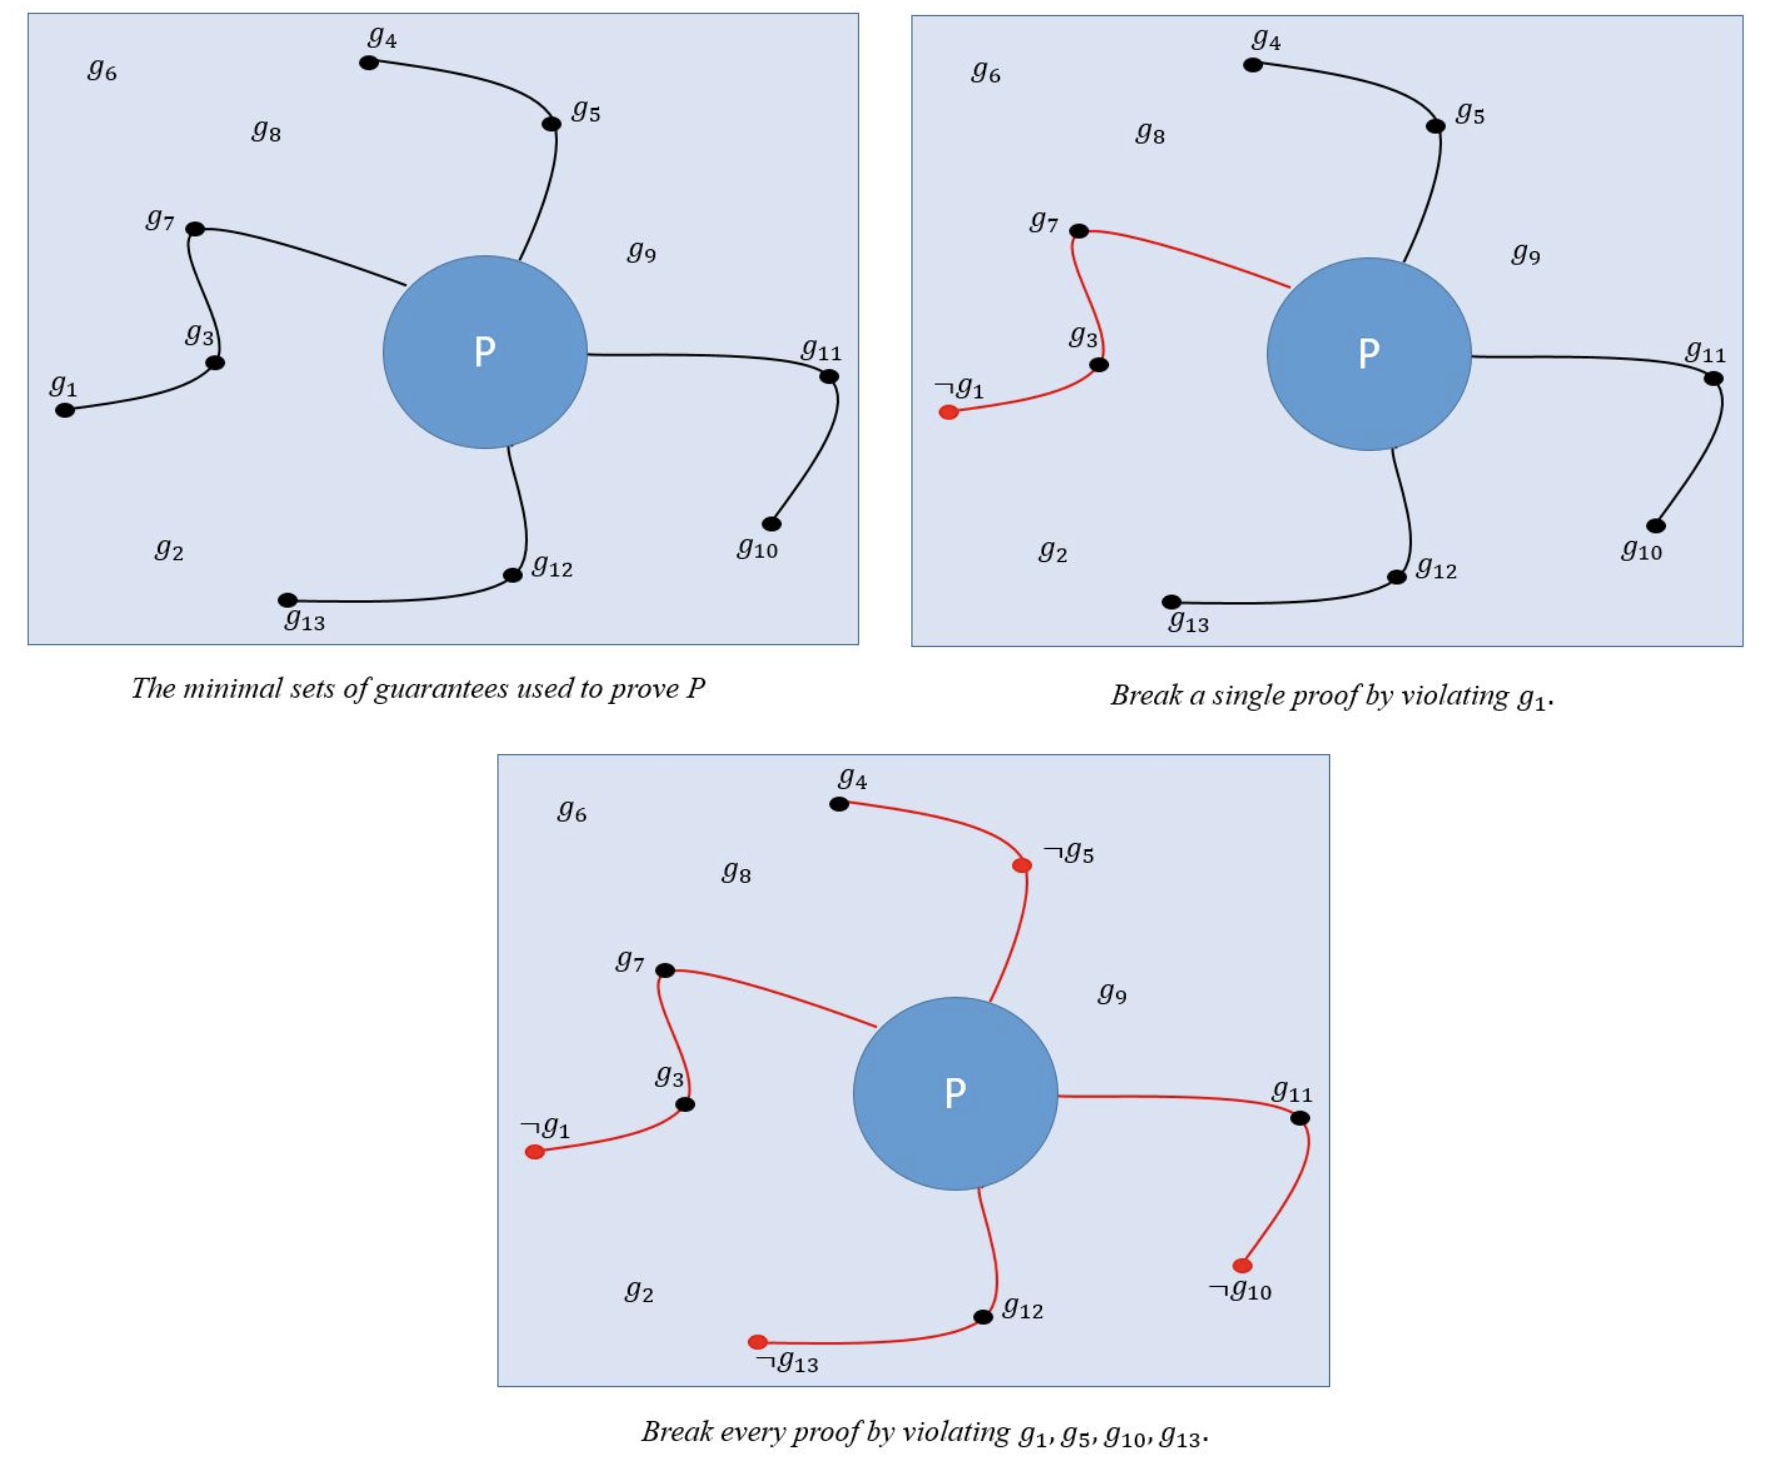
\includegraphics[width=0.9\textwidth]{images/mivcBreaking.png}
	\end{center}
	\caption{Using MIVCs to derive minimal cut sets}
	\label{fig:mivcBreaking}
\end{figure}

In Figure~\ref{fig:mivcBreaking}, we depict this graphically. In the first box (top left), the contracts of the single layer system are $g_1, \dots, g_{13}$. In this example, not all guarantees are needed to prove $P$; one may obtain proof of the property by having only $g_4$ and $g_5$ in the model. The \aivcalg algorithm provides all minimal validity cores which is shown as the lines running through the guarantees. 

One may attempt to ``break" a proof by violating a guarantee in a single MIVC as shown in the top right of the figure. This does break a proof, but given there are multiple MIVCs, it is not enough. The bottom figure shows our method: violate one guarantee from each MIVC set to ensure that the property can no longer be proven. The key idea is that the hitting sets of all MIVCs produces the minimal cut sets. 

Next we outline the formal background and toolsuite used in the implementation and then describe the algorithm that is implemented in the safety annex for AADL. 

\subsection{Background}
JKind is an open-source industrial infinite-state inductive model checker for safety properties~\cite{2017arXiv171201222G}. Models and properties in JKind are specified in Lustre~\cite{Halbwachs91:IEEE}, a synchronous dataflow language, using the theories of linear real and integer arithmetic. JKind uses SMT-solvers to prove and falsify multiple properties in parallel. The JKind model checker uses {\em
  $k$-induction} which unrolls the property $P$ over $k$ steps of the
transition system.

\begin{comment}
%For an arbitrary transition system $(I, T)$, computing reachability can be very expensive or even impossible. Thus, we need a more effective way of checking if a safety property $P$ is satisfied by the system. The key idea is to over-approximate reachability. If we can find an over-approximation that implies the property, then the property must hold. Otherwise, the approximation needs to be refined.

A good first approximation for reachability is the property itself.
That is, we can check if the following formulas hold:
\begin{gather}
  \forall s.~ I(s) \Rightarrow P(s)
  \label{eq:1-ind-base} \\
  \forall s, s'.~ P(s) \land T(s, s') \Rightarrow P(s')
  \label{eq:1-ind-step}
\end{gather}
If both formulas hold then $P$ is {\em inductive} and holds over the
system. If (\ref{eq:1-ind-base}) fails to hold, then $P$ is violated
by an initial state of the system. If (\ref{eq:1-ind-step}) fails to
hold, then $P$ is too much of an over-approximation and needs to be
refined.


The JKind model checker uses {\em
  $k$-induction} which unrolls the property $P$ over $k$ steps of the
transition system. For example, 1-induction consists of formulas (\ref{eq:1-ind-base}) and (\ref{eq:1-ind-step}) above, whereas 2-induction consists of the following formulas:
\begin{gather*}
\forall s.~ I(s) \Rightarrow P(s) \\
\forall s, s'.~ I(s) \land T(s, s') \Rightarrow P(s') \\
\forall s, s', s''.~ P(s) \land T(s, s') \land P(s') \land T(s',
  s'') \Rightarrow P(s'')
\end{gather*}
That is, there are two base step checks and one inductive step check.
In general, for an arbitrary $k$, $k$-induction consists of $k$
base step checks and one inductive step check as shown in
Figure~\ref{fig:k-induction} (the universal quantifiers on $s_i$ have
been elided for space). We say that a property is $k$-inductive if it
satisfies the $k$-induction constraints for the given value of $k$.
The hope is that the additional formulas in the antecedent of the
inductive step make it provable.

\begin{figure}
\begin{gather*}
I(s_0) \Rightarrow P(s_0) \\[-2pt]
%
\vdots \\[2pt]
%
I(s_0) \land T(s_0, s_1) \land \cdots \land T(s_{k-2}, s_{k-1})
\Rightarrow P(s_{k-1}) \\[2pt]
%
P(s_0) \land T(s_0, s_1) \land \cdots \land P(s_{k-1}) \land
T(s_{k-1}, s_k) \Rightarrow P(s_k)
\end{gather*}
\caption{$k$-induction formulas: $k$ base cases and one inductive
  step}
\label{fig:k-induction}
\end{figure}

In practice, inductive model checkers often use a combination of the
above techniques. Thus, a typical conclusion is of the form ``$P$ with
lemmas $L_1, \ldots, L_n$ is $k$-inductive''.
\end{comment}

Each step of induction is sent to an SMT (Satisfiabilty Modulo Theory)-solver to check for \emph{satisfiability}, i.e. there exists a total truth assignment to a given formula that evaluates to true. If there does not exist such an assignment, the formula is considered \emph{unsatisfiable}. %A \emph{constraint system} is a term used to describe the formula with all constraints to the variables. 
A $\mathit{k}$-induction model checker utilizes parallel SMT-solving engines at each induction step to glean information about the proof of a safety property. The transition formula is translated into clauses such that satisfiability is preserved~\cite{een2003temporal}. Expression of the base and induction steps of a temporal induction proof as SAT problems is straightforward and is shown below for step $k$:

\begin{gather*}
I(s_0) \land T(s_0, s_1) \land \cdots \land T(s_{k-1}, s_{k})
\land \neg P(s_{k})
\end{gather*}

When proving correctness it is shown that the formulas are \emph{unsatisfiable}, i.e., the property $P$ is provable. The idea behind finding an {\em inductive validity core} (IVC) for a given property $P$~\cite{GhassabaniGW16} is based on inductive proof methods used in SMT-based model checking, such as $\mathit{k}$-induction and IC3/PDR~\cite{een2011efficient, kahsai2012incremental, cook1971complexity}. Generally, an IVC computation technique aims to determine, for any subset $S \subseteq T$, whether $\mathit{P}$ is provable by $\mathit{S}$. A minimal subset that satisfies $\mathit{P}$ is seen as a minimal proof explanation and called a minimal inductive validity core. %Ghassabani et al. demonstrate that the minimization process is as hard as model checking~\cite{Ghassabani2017EfficientGO}, so finding a minimal inductive validity core may not be possible for some model checking problems. 

\begin{definition}
Inductive Validity Core (IVC)~\cite{GhassabaniGW16}: $S \subseteq T$ for $(I, T) \vdash P$ is an Inductive Validity Core, denoted by $\mathit{IVC(P,S)}$, iff $\mathit{(I,S)} \vdash P$.
\end{definition}

\begin{definition}
Minimal Inductive Validity Core (MIVC)~\cite{Ghassabani2017EfficientGO}: $S \subseteq T$ is a minimal Inductive Validity Core, denoted by $\mathit{MIVC(P,S)}$, iff $\mathit{IVC(P,S)} \land \forall T_i \in S$. $(I, S \setminus \{T_i\}) \not \vdash P$.
\end{definition}

The {\em constraint system} consists of the constrained formulas of the transition system and the negation of the property. The \aivcalg algorithm collects all {\em minimal unsatisfiable subsets} (MUSs) of a constraint system generated from a transition system at each induction step~\cite{Ghassabani2017EfficientGO,bendik2018online}. 

\begin{definition}
A Minimal Unsatisfiable Subset (MUS)~\cite{reiter1987theory} $M$ of a constraint system $C$ is a set $M \subseteq C$ such that $M$ is unsatisfiable and $\forall c \in M$ : $M \setminus \{c\}$ is satisfiable.
\end{definition}
The MUSs are the minimal explanation of the infeasibility of this constraint system; equivalently, these are the minimal sets of model elements necessary for proof of the safety property.

Returning to our running example, this can be illustrated by the following. Given the constraint system $C = \{G_p, G_t, G_r, \neg P\}$, a minimal explanation of the infeasability of this system is the set $\{G_p, G_t, G_r,\}$. If all three guarantees hold, then $P$ (the disjunction of these guarantees) is provable. 

In the case of an UNSAT system, we may ask: what will correct this unsatisfiability? A related set answers this question: 
\begin{definition}
A Minimal Correction Set (MCS)~\cite{reiter1987theory} $M$ of a constraint system $C$ is a subset $M\subseteq C$ such that $C \setminus M$ is satisfiable and $\forall M' \subset M$ : $C \setminus M'$ is unsatisfiable.
\end{definition}
A MCS can be seen to ``correct'' the infeasability of the constraint system by the removal from $C$ the constraints found in an MCS. Returning to the PWR example, the MCSs of the constraint system $C$ are $\mathit{MCS}_1 = \{G_t\}$, $\mathit{MCS}_2 = \{G_p\}$, $\mathit{MCS}_3 = \{G_r\}$. If any single guarantee is violated, a shut down from that subsystem may not get sent when it should and the safety property $P$ will be violated. This corresponds exactly to the definition of a minimal cut set.

For the following definitions, we remind readers of the extended transition system defined in Equation 2 of Section~\ref{sec:formalization} and that the elements of $T$ are the set $\mathit{GF} \cup \mathit{AF}$ for potentially faulty guarantees $\mathit{GF}$ and activation literals $\mathit{AF}$. We use the notation $\mathit{af} \rightarrow \{\mathit{true}, \mathit{false}\}$ to indicate a constraint on the literal $\mathit{af}$. 

\begin{definition}
A cut set $S$ of a top level event $\neg P$ is a set $S \subseteq \mathit{AF}$ such that $\forall \mathit{af} \in S$, $\mathit{af} \rightarrow \{\mathit{true}\}$ and $S \cup \{\neg P\}$ is satisfiable.
\end{definition}

Intuitively, a cut set is a true valuation for some subset of fault activation literals within a constraint system such that the constraint system is satisfiable given those true valuations.

\begin{definition}
A cut set $S$ is minimal if and only if $\forall \mathit{af} \in S$, $S \setminus \{\mathit{af}\} \cup \{\neg P\}$ is unsatisfiable.
\end{definition}

Our approach in computing minimal cut sets through the use of inductive validity cores is to supply activation literals constrained to be false to the algorithm. The resulting $\mathit{MCS}s$ consist of elements $\neg \mathit{af}_i$. The removal of this constraint from the constraint system results in non-deterministically true activation literals. By the definition of an $\mathit{MCS}$, we know that $C \setminus \mathit{MCS}$ is satisifiable. This removal of constraints from $C$ removes the {\em false} constraint from each element in the $\mathit{MCS}$. Liffiton et. al showed that any subset of a satisfiable set is also satisfiable~\cite{liffiton2016fast}, so we know that for set $S$ consisting of elements of $\mathit{MCS}$ with constraints removed, $S \cup \{\neg P\}$ is also satisfiable. This is the definition of a cut set. Minimality comes directly from the definition of a minimal correction set. 

A duality exists between the MUSs of a constraint system and the MCSs as established by Reiter \cite{reiter1987theory}. This duality is defined in terms of \textit{Minimal Hitting Sets} (\textit{MHS}). 
\begin{definition}
A hitting set of a collection of sets $A$ is a set $H$ such that every set in $A$ is ``hit'' by $H$; $H$ contains at least one element from every set in $A$. 
\end{definition}
Every MUS of a constraint system is a minimal hitting set of the system's MCSs, and likewise every MCS is a minimal hitting set of the system's MUSs. This is noted in previous work~\cite{liffiton2016fast, de1987diagnosing} and the proof of such is given by Reiter (Theorem 4.4 and Corollary 4.5)~\cite{reiter1987theory}. For the PWR top level constraint system, it can be seen that each of the MCSs intersected with the MUS is nonempty. This gives the minimal set of guarantees for which, if violated, will cause $P$ to be violated. 

As described in Section~\ref{sec:formalization}, we extend the transition system with fault activation literals. These literals are constrained to {\em false} and the \aivcalg algorithm is invoked. The constraint system for the PWR example is $C = \{\neg\mathit{af}_p, \neg\mathit{af}_t, \neg\mathit{af}_r, \neg P\}$ for activation literal $\mathit{af}_p$ associated with $G_p$, etc. The hitting sets generated from the MIVC are: $\{\neg\mathit{af}_p\}$, $\{\neg\mathit{af}_t\}$, and $\{\neg\mathit{af}_r\}$ and are the minimal correction sets of the constraint system. 

%\textbf{Background Information on Toolsuite}
\danielle{My suggestion is to place this at the front of the implementation section. It just seems like it is taking longer to get to the interesting part of the paper by having it here.}

The algorithms in this paper are implemented in the Safety Annex for the Architecture Analysis and Design Language (AADL) and require the Assume-Guarantee Reasoning Environment (AGREE)~\cite{NFM2012:CoGaMiWhLaLu} to annotate the AADL model in order to perform verification using the back-end model checker \jkind~\cite{2017arXiv171201222G}. 

\textbf{Architecture Analysis and Design Language}
We are using the Architectural Analysis and Design Language (AADL) to construct system architecture models of performance-critical, embedded, real-time systems~\cite{AADL_Standard,FeilerModelBasedEngineering2012}. %An AADL model describes a system in terms of a hierarchy of components and their interconnections, where each component can either represent a logical entity (e.g., application software functions, data) or a physical entity (e.g., buses, processors). 
Language annexes to AADL provide a richer set of modeling elements for various system design and analysis needs, and the language definition is sufficiently rigorous to support formal analysis tools that allow for early phase error/fault detection. 

\textbf{Compositional Analysis} 
One way to structure compositional verification is hierarchically: layers of the system architecture are analyzed independently and their composition demonstrates a system property of interest. Compositional verification partitions the formal analysis of a system architecture into verification tasks that correspond into the decomposition of the architecture~\cite{clarke1989compositional}.  A proof consists of demonstrating that the system property is provable given the contracts of its direct subcomponents and the system assumptions~\cite{cofer2012compositional,clarke1989compositional}. When compared to monolithic analysis (i.e., analysis of the flattened model composed of all components), the compositional approach allows the analysis to scale to much larger systems~\cite{NFM2012:CoGaMiWhLaLu,heckel1998compositional,cofer2012compositional}.

\textbf{Assume Guarantee Reasoning Environment}
The Assume Guarantee Reasoning Environment (AGREE) is a tool for formal analysis of behaviors in AADL models and supports compositional verification~\cite{NFM2012:CoGaMiWhLaLu}.  It is implemented as an AADL annex and is used to annotate AADL components with formal behavioral contracts. Each component's contracts includes assumptions and guarantees about the component's inputs and outputs respectively. AGREE translates an AADL model and the behavioral contracts into Lustre~\cite{Halbwachs91:IEEE} and then queries the \jkind model checker to conduct the back-end analysis~\cite{2017arXiv171201222G}. 

\textbf{JKind}
JKind is an open-source industrial infinite-state inductive model checker for safety properties~\cite{2017arXiv171201222G}. Models and properties in JKind are specified in Lustre~\cite{Halbwachs91:IEEE}, a synchronous dataflow language, using the theories of linear real and integer arithmetic. JKind uses SMT-solvers to prove and falsify multiple properties in parallel.

\textbf{Safety Annex for AADL}
The Safety Annex for AADL provides the ability to reason about faults and faulty component behaviors in AADL models~\cite{Stewart17:IMBSA,stewart2020safety}. In the Safety Annex approach, AGREE is used to define the nominal behavior of system components, faults are introduced into the nominal model, and JKind is used to analyze the behavior of the system in the presence of faults. Faults describe deviations from the nominal behavior and are attached to the outputs of components in the system.%The Safety Annex supports behavioral specification of faults and their implicit propagation through behavioral relationships in the model as well as explicit propagation through dependencies. 


